% Krino v4 -- listwise marker model on Qwen3.5-4B
% Build: make build   (uses oaklight/texlive:science-cn)
\documentclass[tikz,border=10pt]{standalone}
\usepackage{amsmath}
\usepackage{amssymb}
\usetikzlibrary{arrows.meta,positioning,calc,decorations.pathreplacing,shapes.geometric}

% ---------------------------------------------------------------- palette
\definecolor{frozenfill}{HTML}{F3F4F6}
\definecolor{frozendraw}{HTML}{6B7280}
\definecolor{trainfill}{HTML}{EFF6FF}
\definecolor{trainraw}{HTML}{2563EB}
\definecolor{datafill}{HTML}{F0FDF4}
\definecolor{datadraw}{HTML}{16A34A}
\definecolor{fusefill}{HTML}{F5F3FF}
\definecolor{fusedraw}{HTML}{7C3AED}
\definecolor{lossfill}{HTML}{FFFBEB}
\definecolor{lossdraw}{HTML}{D97706}
\definecolor{markerfill}{HTML}{FEF2F2}
\definecolor{markerdraw}{HTML}{DC2626}
\definecolor{notefill}{HTML}{FAFAF9}
\definecolor{loraFill}{HTML}{FEF3C7}
\definecolor{loraDraw}{HTML}{B45309}

\tikzset{
  box/.style={rounded corners=3pt, draw, line width=0.6pt, align=center,
              inner sep=5pt, font=\sffamily\small},
  frozen/.style={box, fill=frozenfill, draw=frozendraw},
  trainable/.style={box, fill=trainfill, draw=trainraw},
  lora/.style={box, fill=loraFill, draw=loraDraw},
  data/.style={box, fill=datafill, draw=datadraw},
  fusebox/.style={box, fill=fusefill, draw=fusedraw},
  lossbox/.style={box, fill=lossfill, draw=lossdraw},
  note/.style={rounded corners=3pt, draw=black!30, line width=0.5pt,
               fill=notefill, align=flush left, inner sep=5pt,
               font=\sffamily\footnotesize},
  token/.style={draw=frozendraw, fill=white, rounded corners=1.5pt,
                minimum height=0.5cm, inner sep=3pt, font=\sffamily\scriptsize},
  marker/.style={token, draw=markerdraw, fill=markerfill,
                 font=\sffamily\scriptsize\bfseries},
  arrow/.style={-{Stealth[length=2.2mm,width=1.6mm]}, line width=0.6pt,
                draw=black!70},
  dasharrow/.style={arrow, dashed},
  alabel/.style={font=\sffamily\scriptsize, text=black!65, align=center},
}

\begin{document}
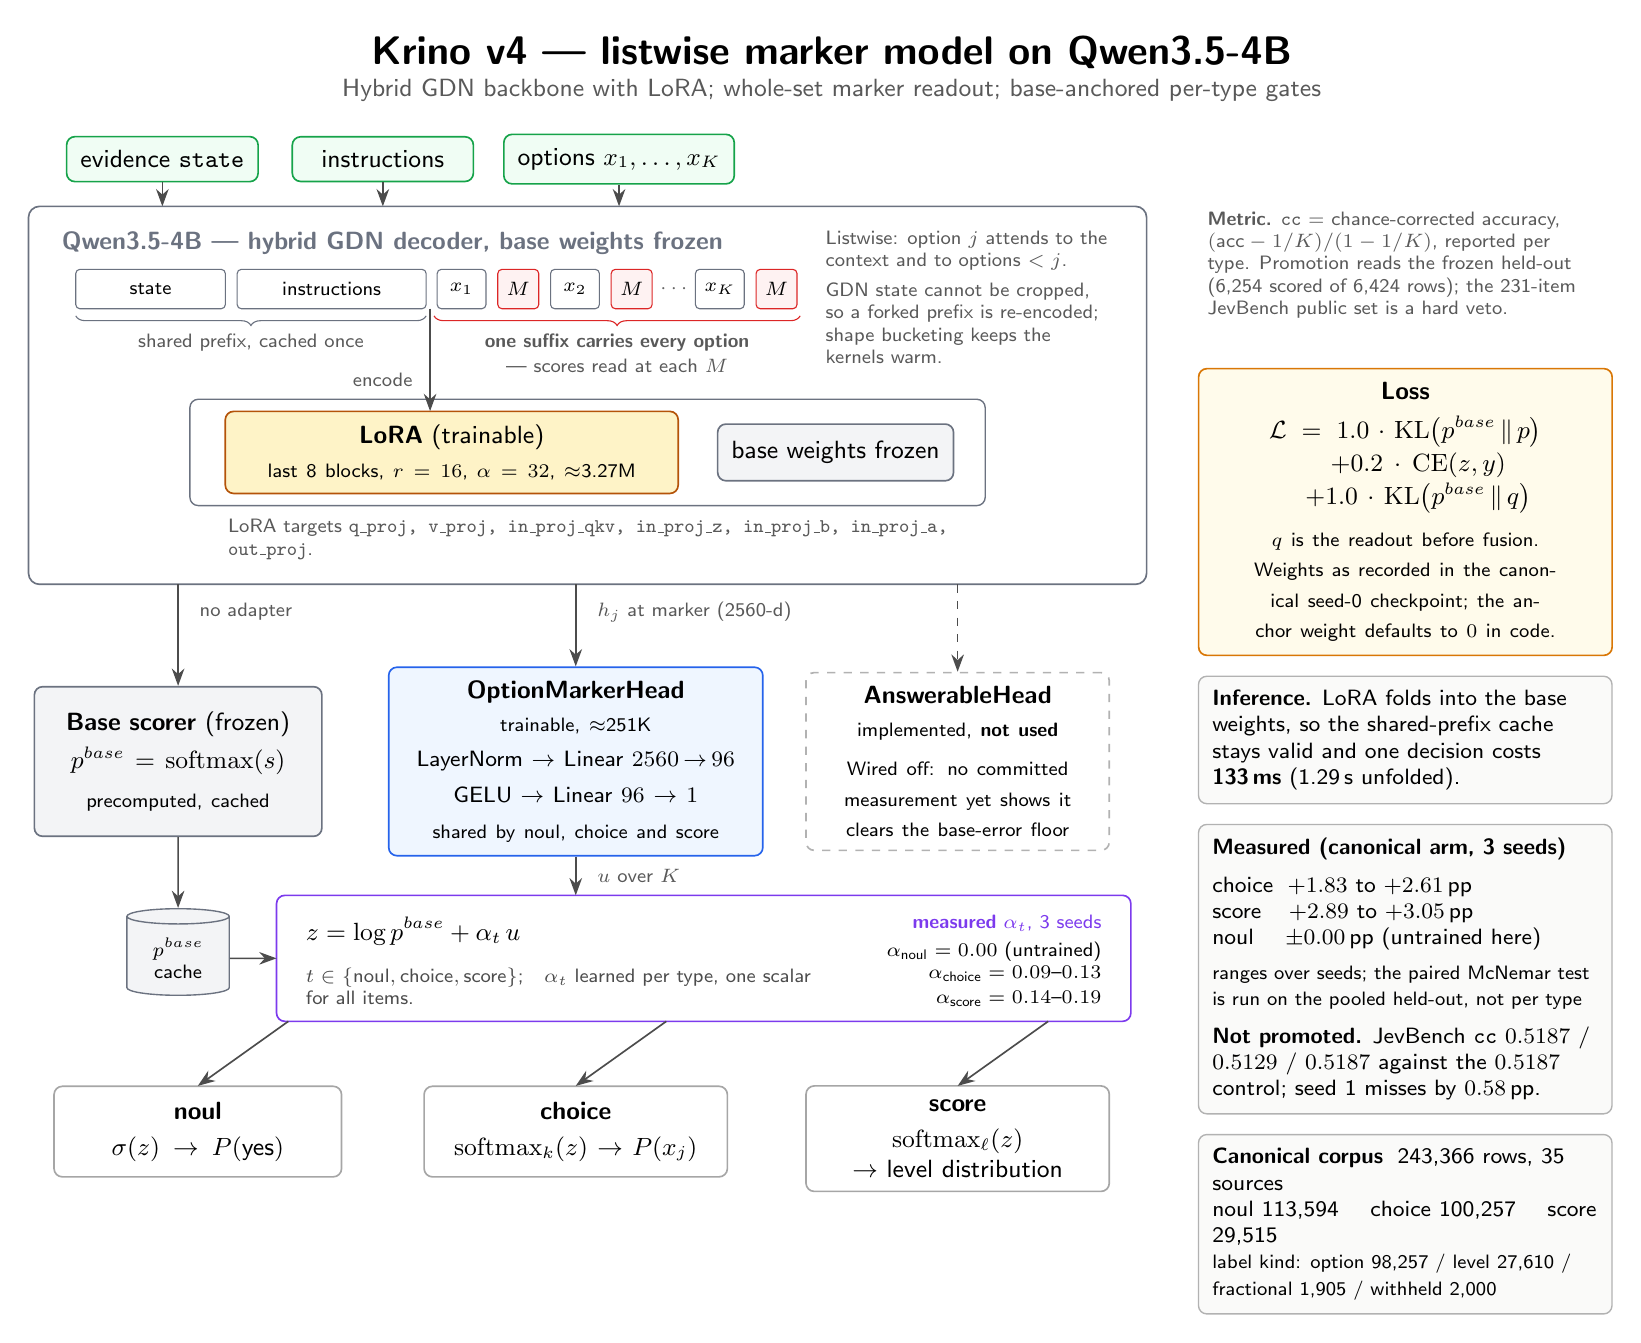
\begin{tikzpicture}[font=\sffamily]

% ================================================================ title
\node[font=\sffamily\Large\bfseries] at (10.6,16.45)
  {\textsf{Krino v4 --- listwise marker model on Qwen3.5-4B}};
\node[font=\sffamily\small, text=black!65] at (10.6,15.98)
  {\textsf{Hybrid GDN backbone with LoRA; whole-set marker readout; base-anchored per-type gates}};

% ================================================================ inputs
\node[data, minimum width=2.0cm] (instate) at (2.1,15.1) {evidence \texttt{state}};
\node[data, minimum width=2.3cm] (ininstr) at (4.9,15.1) {instructions};
\node[data, minimum width=2.6cm] (inopts)  at (7.9,15.1) {options $x_1,\dots,x_K$};
\foreach \n in {instate,ininstr,inopts}
  \draw[arrow] (\n.south) -- (\n.south |- 0,14.5);

% ================================================================ backbone
\draw[frozenfill, draw=frozendraw, line width=0.6pt, rounded corners=4pt]
  (0.4,9.7) rectangle (14.6,14.5);
\node[anchor=north west, font=\sffamily\small\bfseries, text=frozendraw]
  at (0.7,14.3) {Qwen3.5-4B --- hybrid GDN decoder, base weights frozen};

% token strip: shared prefix | listwise suffix
\node[token, minimum width=1.9cm] (tstate) at (1.95,13.45) {state};
\node[token, minimum width=2.4cm] (tinstr) at (4.25,13.45) {instructions};
\node[token, minimum width=0.62cm] (txa) at (5.90,13.45) {$x_1$};
\node[marker, minimum width=0.52cm] (tma) at (6.62,13.45) {$M$};
\node[token, minimum width=0.62cm] (txb) at (7.34,13.45) {$x_2$};
\node[marker, minimum width=0.52cm] (tmb) at (8.06,13.45) {$M$};
\node[font=\sffamily\scriptsize, text=black!60] at (8.62,13.45) {$\cdots$};
\node[token, minimum width=0.62cm] (txk) at (9.18,13.45) {$x_K$};
\node[marker, minimum width=0.52cm] (tmk) at (9.90,13.45) {$M$};

\draw[decorate, decoration={brace, amplitude=3.5pt, raise=2pt, mirror}, draw=frozendraw]
  (1.00,13.18) -- (5.45,13.18)
  node[midway, below=5pt, font=\sffamily\scriptsize, text=black!65]
  {shared prefix, cached once};
\draw[decorate, decoration={brace, amplitude=3.5pt, raise=2pt, mirror}, draw=markerdraw]
  (5.55,13.18) -- (10.20,13.18)
  node[midway, below=5pt, font=\sffamily\scriptsize, text=black!65,
       align=center]
  {\textbf{one suffix carries every option}\\[1pt]
   --- scores read at each $M$};

\node[anchor=west, font=\sffamily\scriptsize, text=black!65, align=flush left,
      text width=3.6cm] at (10.40,13.35)
  {Listwise: option $j$ attends to the context and to options $<j$.\\[3pt]
   GDN state cannot be cropped, so a forked prefix is re-encoded; shape
   bucketing keeps the kernels warm.};

% adapted weights: LoRA adapters and the frozen base are one unit
\draw[draw=frozendraw, line width=0.5pt, rounded corners=3pt]
  (2.45,10.70) rectangle (12.55,12.05);

\node[lora, text width=5.4cm, minimum height=0.72cm] (lora) at (5.775,11.375)
  {\textbf{LoRA} (trainable)\\[1pt]
   {\scriptsize last 8 blocks, $r=16$, $\alpha=32$, $\approx$3.27M}};
\node[frozen, minimum width=2.9cm, minimum height=0.72cm] (blocks) at (10.65,11.375)
  {base weights frozen};

\draw[arrow] (5.50,13.20) -- (5.50,11.90);
\node[alabel, anchor=east] at (5.40,12.30) {encode};

\node[anchor=west, font=\sffamily\scriptsize, text=black!65, align=flush left,
      text width=9.4cm] at (2.81,10.27)
  {LoRA targets \texttt{q\_proj, v\_proj, in\_proj\_qkv, in\_proj\_z,
   in\_proj\_b, in\_proj\_a, out\_proj}.};

% ================================================================ head row
\node[frozen, text width=3.3cm, minimum height=1.9cm] (base) at (2.30,7.45)
  {\textbf{Base scorer} (frozen)\\[3pt]
   $p^{base}=\operatorname{softmax}(s)$\\[3pt]
   {\scriptsize precomputed, cached}};
\draw[arrow] (2.30,9.7) -- (base.north);
\node[alabel, anchor=west] at (2.45,9.35) {no adapter};

\node[trainable, text width=4.4cm, minimum height=1.9cm] (markerhead) at (7.35,7.45)
  {\textbf{OptionMarkerHead}\\[1pt]
   {\scriptsize trainable, $\approx$251K}\\[3pt]
   {\footnotesize LayerNorm $\to$ Linear $2560\!\to\!96$\\[2pt]
   GELU $\to$ Linear $96\!\to\!1$}\\[2pt]
   {\scriptsize shared by noul, choice and score}};
\draw[arrow] (7.35,9.7) -- (markerhead.north);
\node[alabel, anchor=west] at (7.50,9.35) {$h_j$ at marker (2560-d)};

\node[box, draw=black!30, fill=white, dashed, text width=3.5cm, minimum height=1.9cm]
  (anshead) at (12.20,7.45)
  {\textbf{AnswerableHead}\\[1pt]
   {\scriptsize implemented, \textbf{not used}}\\[3pt]
   {\scriptsize Wired off: no committed measurement yet shows it clears the
    base-error floor}};
\draw[dasharrow] (12.20,9.7) -- (anshead.north);

% ================================================================ p_base cache
\node[cylinder, draw=frozendraw, fill=frozenfill, line width=0.5pt,
      shape border rotate=90, aspect=0.22,
      minimum width=1.3cm, minimum height=1.1cm,
      font=\sffamily\scriptsize, align=center] (cache) at (2.30,4.95)
  {$p^{base}$\\cache};
\draw[arrow] (base.south) -- (cache.north);

% ================================================================ fusion
\draw[fusefill, draw=fusedraw, line width=0.6pt, rounded corners=3pt]
  (3.55,4.15) rectangle (14.40,5.75);
\node[anchor=north west, font=\sffamily\small] at (3.80,5.60)
  {$\displaystyle z=\log p^{base}+\alpha_t\,u$};
\node[anchor=north west, font=\sffamily\scriptsize, text=black!70,
      text width=6.6cm, align=flush left] at (3.80,4.95)
  {$t\in\{\text{noul},\text{choice},\text{score}\}$;\quad
   $\alpha_t$ learned per type, one scalar for all items.};
\node[anchor=north east, font=\sffamily\scriptsize, align=right] at (14.15,5.62)
  {{\scriptsize\color{fusedraw}\textbf{measured} $\alpha_t$, 3 seeds}\\[2pt]
   $\alpha_{\text{noul}}=0.00$ (untrained)\\
   $\alpha_{\text{choice}}=0.09$--$0.13$\\[1pt]
   $\alpha_{\text{score}}=0.14$--$0.19$};

\draw[arrow] (cache.east) -- (3.55,4.95);
\draw[arrow] (markerhead.south) -- (7.35,5.75);
\node[alabel, anchor=west] at (7.50,6.00) {$u$ over $K$};

% ================================================================ outputs
\node[box, draw=black!35, fill=white, text width=3.3cm, minimum height=1.15cm]
  (outnoul) at (2.55,2.75)
  {\textbf{noul}\\[2pt] $\sigma(z)\to P(\text{yes})$};
\node[box, draw=black!35, fill=white, text width=3.5cm, minimum height=1.15cm]
  (outchoice) at (7.35,2.75)
  {\textbf{choice}\\[2pt] $\operatorname{softmax}_k(z)\to P(x_j)$};
\node[box, draw=black!35, fill=white, text width=3.5cm, minimum height=1.15cm]
  (outscore) at (12.20,2.66)
  {\textbf{score}\\[2pt] $\operatorname{softmax}_\ell(z)$\\ $\to$ level distribution};

\draw[arrow] (3.70,4.15) -- (2.55,3.33);
\draw[arrow] (8.50,4.15) -- (7.35,3.33);
\draw[arrow] (13.35,4.15) -- (12.20,3.33);

% ================================================================ right column
\node[anchor=north west, font=\sffamily\scriptsize, text=black!65,
      text width=4.9cm, align=flush left] at (15.25,14.55)
  {\textbf{Metric.} \texttt{cc} = chance-corrected accuracy,
   $(\text{acc}-1/K)/(1-1/K)$, reported per type. Promotion reads the frozen
   held-out (6{,}254 scored of 6{,}424 rows); the 231-item JevBench public set
   is a hard veto.};

\node[lossbox, anchor=north west, text width=4.9cm] (loss) at (15.25,12.45)
  {\textbf{Loss}\\[3pt]
   $\mathcal{L}=1.0\cdot\mathrm{KL}\!\left(p^{base}\,\|\,p\right)$\\[1pt]
   $\quad+0.2\cdot\mathrm{CE}(z,y)$\\[1pt]
   $\quad+1.0\cdot\mathrm{KL}\!\left(p^{base}\,\|\,q\right)$\\[4pt]
   {\scriptsize $q$ is the readout before fusion. Weights as recorded in the
    canonical seed-0 checkpoint; the anchor weight defaults to $0$ in code.}};

\node[note, anchor=north west, text width=4.9cm] (infer) at ([yshift=-7pt]loss.south west)
  {\textbf{Inference.} LoRA folds into the base weights, so the shared-prefix
   cache stays valid and one decision costs \textbf{133\,ms} (1.29\,s
   unfolded).};

\node[note, anchor=north west, text width=4.9cm] (results) at ([yshift=-7pt]infer.south west)
  {\textbf{Measured (canonical arm, 3 seeds)}\\[4pt]
   choice $\;+1.83$ to $+2.61$\,pp\\
   score $\;\;\;+2.89$ to $+3.05$\,pp\\
   noul $\quad\pm0.00$\,pp (untrained here)\\[3pt]
   {\scriptsize ranges over seeds; the paired McNemar test is run on the
    pooled held-out, not per type}\\[4pt]
   \textbf{Not promoted.} JevBench \texttt{cc} $0.5187$ / $0.5129$ / $0.5187$
   against the $0.5187$ control; seed 1 misses by $0.58$\,pp.};

\node[note, anchor=north west, text width=4.9cm] (data) at ([yshift=-7pt]results.south west)
  {\textbf{Canonical corpus} \;243{,}366 rows, 35 sources\\
   noul 113{,}594 \quad choice 100{,}257 \quad score 29{,}515\\
   {\scriptsize label kind: option 98{,}257 / level 27{,}610 /
    fractional 1{,}905 / withheld 2{,}000}};

\end{tikzpicture}
\end{document}
